\documentclass[paper=letter, fontsize=12pt]{article}

\usepackage[english]{babel}
\usepackage{amsmath,amssymb}
\usepackage[utf8]{inputenc}
\usepackage{graphicx,url}
\usepackage[labelsep=period]{caption}  
\usepackage{tikz}
\usepackage{subfigure}
\usepackage{bm,bbm}
\usepackage[hmarginratio=1:1,top=32mm,columnsep=20pt]{geometry} 
\usepackage{booktabs}
\usepackage[colorlinks=true, urlcolor=blue,  linkcolor=blue, citecolor=blue]{hyperref}
\usepackage{abstract}
\usepackage{fancyhdr} 
\usepackage{setspace}
\usepackage{color}

\renewcommand{\abstractnamefont}{\normalfont\bfseries}
\renewcommand{\abstracttextfont}{\normalfont\small\itshape}

\newcommand{\horrule}[1]{\rule{\linewidth}{#1}}
\pagestyle{fancy}
\fancyhead{} 
\fancyfoot{} 

\fancyhead[C]{Universidade Federal de Minas Gerais $\bullet$ Departamento de Ciência da Computação %~ $\bullet$ 1ª semestre de 2018 
} 

\fancyfoot[RO,LE]{\thepage}

\captionsetup{justification=centering,font=normal} 
\captionsetup[figure]{font=small}

\usepackage{color}

\hyphenation{}

\newdimen\HilbertLastX
\newdimen\HilbertLastY
\newcounter{HilbertOrder}

\def\DrawToNext#1#2{%
   \advance \HilbertLastX by #1
   \advance \HilbertLastY by #2
   \pgfpathlineto{\pgfqpoint{\HilbertLastX}{\HilbertLastY}}
   % Alternative implementation using plot streams:
   % \pgfplotstreampoint{\pgfqpoint{\HilbertLastX}{\HilbertLastY}}
}

% \Hilbert[right_x,right_y,left_x,left_x,up_x,up_y,down_x,down_y]
\def\Hilbert[#1,#2,#3,#4,#5,#6,#7,#8] {
  \ifnum\value{HilbertOrder} > 0%
     \addtocounter{HilbertOrder}{-1}
     \Hilbert[#5,#6,#7,#8,#1,#2,#3,#4]
     \DrawToNext {#1} {#2}
     \Hilbert[#1,#2,#3,#4,#5,#6,#7,#8]
     \DrawToNext {#5} {#6}
     \Hilbert[#1,#2,#3,#4,#5,#6,#7,#8]
     \DrawToNext {#3} {#4}
     \Hilbert[#7,#8,#5,#6,#3,#4,#1,#2]
     \addtocounter{HilbertOrder}{1}
  \fi
}

% \hilbert((x,y),order)
\def\hilbert((#1,#2),#3){%
   \advance \HilbertLastX by #1
   \advance \HilbertLastY by #2
   \pgfpathmoveto{\pgfqpoint{\HilbertLastX}{\HilbertLastY}}
   % Alternative implementation using plot streams:
   % \pgfplothandlerlineto
   % \pgfplotstreamstart
   % \pgfplotstreampoint{\pgfqpoint{\HilbertLastX}{\HilbertLastY}}
   \setcounter{HilbertOrder}{#3}
   \Hilbert[1mm,0mm,-1mm,0mm,0mm,1mm,0mm,-1mm]
   \pgfusepath{stroke}%
}

\title{\vspace{-10mm}\fontsize{24pt}{10pt}\selectfont\textbf{ 
Dissertation Proposal \\ \vspace{8mm} \normalfont{A study about ordinal patterns transition graphs}}} 
\author{
\large
{\textsc{Eduarda Tatiane Caetano Chagas}}\\[2mm]
{\textsc{Advisor: Heitor S.\ Ramos}}\\[2mm]
{\textsc{Co-advisor: Alejandro C.\ Frery}}\\[2mm]
\normalsize {\{eduarda.chagas, ramosh\}@dcc.ufmg.br, acfrery@laccan.ufal.br}\\[2mm]
}
\date{}


\begin{document}
\maketitle 
\thispagestyle{fancy}

\onehalfspacing 

\section{Introduction}~\label{sec:introduction}

The main hypothesis underlying this dissertation project can be briefly stated as follows:

\begin{quote}

    Ordinal pattern transition graphs capture intrinsic characteristics of the time series underlying phenomena and capture information about system dynamics in finer granularity.
    
\end{quote}
%\todo[inline]{Vê se não fica melhor assim: Ordinal pattern transition graphs capture intrinsic characteristics of the time series underlying phenomena and capture information about system dynamics in finer granularity.}
%DONE

\textcolor{red}{Fazer uma transição de s\'erie temporal a imagens}

Therefore, we plan to evaluate the power of characterization and consequently of image classification when we analyze them as ordinal patterns transition graphs.

The following sections motivate, support, and detail this dissertation project.
This work was divided as follows:
Section~\ref{sec:motivation} exposes the motivations of this study.
Section~\ref{methodology} presents the proposed methodology.
Section~\ref{linearization} reports how the patch linearization process of the images occurs.
Section~\ref{WATG} describes our technique of ordinal amplitude transition graph weighting by amplitudes.
In Section~\ref{HC} we report the Information Theory descriptors used throughout this work.
Section~\ref{sec:results} shows the expected results with the dissertation proposal presented.
Section~\ref{sec:checkpoint} we present the schedule to be followed.
We present our conclusions in Section~\ref{sec:final}.


\section{Motivation}~\label{sec:motivation}

Surface classification and land use are among the most important applications of Synthetic Aperture Radar (SAR) imaging \cite{Pottier2004Unsupervised}, for which supervised and unsupervised classification algorithms have been proposed~\cite{Chen1996multifrequency,Bhattacharya2018Unsupervised,ZYL1992Bayesian}.

Classification techniques rely on the extraction and analysis of features from the data, and from additional information and prior knowledge about  the scene, the sensor and the acquisition conditions.
Texture is among the features that carries most information and, as such, it is important to characterize it in a quantitative manner.

The texture in SAR images is characterized twofold, namely by the marginal properties of the data~\cite{adrian96}, and by their spatial structure~\cite{FeaturesCropDiscrimination}.
In this work we focus on the second approach.

The most widely used approach to obtain textural features from SAR imagery is through co-ocurrence matrices and Haralick's descriptors~\cite{Zakeri2017Texture}.
Other approaches include the Fourier power spectrum~\cite{Florindo2012Fractal}, and
Markov random fields~\cite{Deng2005UnsupervisedSO}.

In our approach, we chose to linearize the image patches and analyze the resulting 1-D signals as time series.
By doing that, we reduce the data dimensionality and map the spatial dependence of pixels into a temporal correlation.
Then, starting from the ordinal patterns from the time series, we propose a novel weighted graph of pattern transitions that is able to discriminate patterns corresponding to different amplitude levels.
Finally, we will use well-known features from information theory to characterize image patches.
%\todo[inline]{os verbos estão todos no passado, já terminou o trabalho?}
%DONE
	
This dissertation proposes and analyzes a novel technique for SAR image texture characterization that is based on a modified version of ordinal pattern transition graphs.
This approach is able to discriminate similar patterns with different amplitude levels. 
	
\section{Methodology}\label{methodology}

Figure~\ref{fig:WATG} presents a schematic view of this dissertation proposal. 
In the following, we present a more detailed discussion of each element.
%%% ACF Não deixe linha em branco entre elementos que formam o mesmo parágrafo
\begin{enumerate}
	\item\label{item:Linearlize} Transforming a 2-D patch of data into a time series using a Hilbert Space Filling Curve,
	\item\label{item:WOPTG} Building an Ordinal Pattern Transition Graph with weighted edges;
	\item\label{item:Probability} Obtaining a probability distribution function from this graph;
	\item\label{item:Descriptors} Computing the Entropy and Statistical Complexity of this distribution.
\end{enumerate}

	
\begin{figure}[hbt]
	\centering
	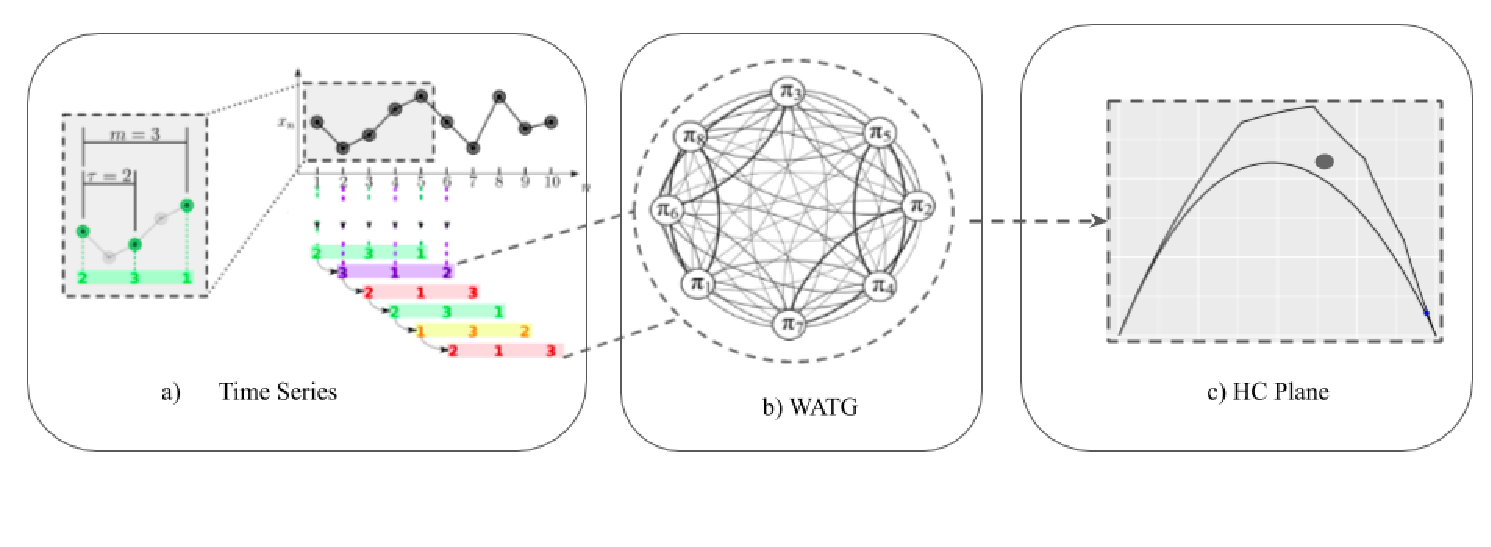
\includegraphics[width=\linewidth]{Figures/WATG.pdf}
	\vspace{-.8cm}
	\caption{Outline of the technique for the characterization of textures.}
	\label{fig:WATG}
\end{figure}

\subsection{Linearization of image patches}\label{linearization}

In this step, we perform a data dimensionality reduction by turning 2-D patches into 1-D signals.
For this, we opt to do a linearization of the data through techniques that maintain the spatial correlation of the image.
This could be accomplished by reading the data by lines, columns or any transformation.
In Step~\ref{item:Linearlize} we employ a Hilbert Space Filling Curve~\cite{Lee1994Texture}.

Space filling curves were first employed by Nguyen and Quinqueton (1982), to map a texture into a one-dimensional signal.
When used as scanning methods of an image, such functions preserve relevant properties of pixel spatial correlation~\cite{Lee1994Texture}.

Assuming an image patch is supported by a $N \times N$ dimension grid, where $N$ is a power of $2$, we have the following definition.

\newtheorem{mydef}{Definition}
\begin{mydef}
	An image scan is a bijective function $f \colon \mathbb{N} \times \mathbb{N} \to \mathbb{N}$ defined in the ordered pair set $ \{(i, j): 1 \leq i , j \leq N \}$, which uniquely indexes the points in the domain in the closed range of integers $\{1, \dots, N^2\}$.
	A scan rule is $\{f^{-1}(1), \dots, f^{-1}(N^2)\}$.
	\label{def:CurveFilling}
\end{mydef}
This Definition imposes that each pixel is visited only once.

Space filling curves, such as raster-1, raster-2 and Hilbert scanning techniques stipulate a proper function $f$.
%%% ACF Ilustre raster-1 e raster-2
Hilbert curves scans an array of pixels of dimension $2^k \times 2^k$, $k \in \mathbb{N}$, never keeping the same direction for more than three consecutive points, as shown in Figure~\ref{fig:Hilbert}.
Using a Hilbert curve we reduce the data dimensionality by maintaining the spatial dependence information of the analyzed textures.

\begin{figure}[hbt]
	\centering
	\tikz[scale=3.6] \hilbert((0mm,0mm),3);
	\hspace{0.3cm}
	\tikz[scale=1.7] \hilbert((0mm,0mm),4);
	\hspace{0.3cm}
	\tikz[scale=0.85] \hilbert((0mm,0mm),5);	
	\caption{Hilbert space filling curve in areas of: (a) $8 \times 8$, (b) $16 \times 16$ and (c) $32 \times 32$. }\label{fig:Hilbert}
	%%% ACF Aumente a escala das figuras; ocupe toda a largura da linha
\end{figure} 

%%% ACF Talvez valha a pena pensar em *quatro* etapas: (i) linearização, (ii) ordinal patterns, (iii) weighted ordinal patters transition graph, (iv) information theory descriptors. Isso pode ficar para a versão final. Cada etapa poderia estar fartamente ilustrada, o que iria requerer colocar, por exemplo, duas imagens de Brodatz logo no início para ilustrar cada etapa.
\subsection{Weighted Ordinal Patterns Transition Graph}\label{WATG}

Step~\ref{item:WOPTG} consists of two stages.
In the first, the time series is transformed into a sequence of ordinal patterns.
In the second, we build a weighted graph describing the transitions between these patterns.

The representation of time series by ordinal patterns was introduced by~\cite{Bandt2002Permutation} as a transformation resistant to noise, and invariant to nonlinear monotonic transformations.

Consider ${\mathcal X} \equiv \{x_t\}_{t=1}^{T}$ a real valued time series of length $T$. 

Let ${\mathfrak A}_{D}$ (with $D \geq 2$ and $D \in {\Bbb N}$) be the symmetric group of order $D!$ formed by all 
possible permutations of order $D$, and the symbol component vector 
${\bm \pi}^{(D)} = (\pi_1, \pi_2, \dots, \pi_D)$ so every element ${\bm \pi}^{(D)}$ is unique 
($\pi_j \neq \pi_k$ for every $j \neq k$). 

Consider for the time series ${\mathcal X} \equiv \{x_t\}_{t=1}^{T}$ its time delay embedding representation,
with embedding dimension $D \geq 2$ and time delay $\tau \geq 1$ ($\tau \in {\Bbb N}$, also called ``embedding time'', ``time delay'', or ``delay''):
\begin{equation} 
\label{eq:time-delay}
{\mathbf X}^{(D,\tau)}_t ~=)~ x_t,x_{t+\tau},\dots,x_{t+(D-1)\tau} ) ,
\end{equation} 
for $t = 1,2,\dots,N$ with $N = T-(D-1) \tau$.
Then the vector ${\mathbf X}^{(D,\tau)}_t$ can be mapped to a symbol vector ${\bm \pi}_t^D \in {\mathfrak A}_{D}$. 
This mapping should be defined in a way that preserves the desired relation between the elements 
$x_t  \in {\mathbf X}^{(D,\tau)}_t$, and all $t \in \{1,\dots,T-(D-1)\tau\}$ that share this pattern (also called ``motif'') are mapped to the same 
${\bm \pi}_t^{D}$.

Without loss of generality, we define the mapping ${\mathbf X}_t^{(D,\tau)} \mapsto {\mathbf \pi}_t^{D}$ by ordering the observations $x_t \in {\mathbf X}_t^{(D,\tau)}$ in increasing order.
Consider the time series $\mathcal X = (1.8, 1.2, 3.2, 4.8, 4.2, 4.5, 2.3, 3.7, 1.2, .5)$ depicted in Fig.~\ref{Fig:IntroBP}.
Assume we are using patterns of length $D=5$ with unitary time lag $\tau=1$.
The code associated to $\mathbf X_{3}^{(5,1)}=(x_3,\dots,x_7)=(3.2, 4.8, 4.2, 4.5, 2.3)$, shown in black, is formed by the indexes in $\bm\pi_3^{5}=(1,2,3,4,5)$ which sort the elements of $\mathbf X_{3}^{(5,1)}$ in increasing order: $51342$.
With this, $\widetilde{\pi}_3^{5} = 51342$, and we increase the counting related to this motif in the histogram of all possible patterns of size $D=5$.

The dash-dot line in Fig.~\ref{Fig:IntroBP} illustrates $\mathbf X_{1}^{(5,2)}$, i.e. the sequence of length $D=5$ starting at $x_1$ with lag $\tau=2$.
In this case, $\mathbf X_{1}^{(5,2)}= (1.8, 3.2, 4.2, 2.3, 1.2)$, and the corresponding motif is $\widetilde{\pi}_1^{5}=51423$.

\begin{figure}[hbt]
	\centering
	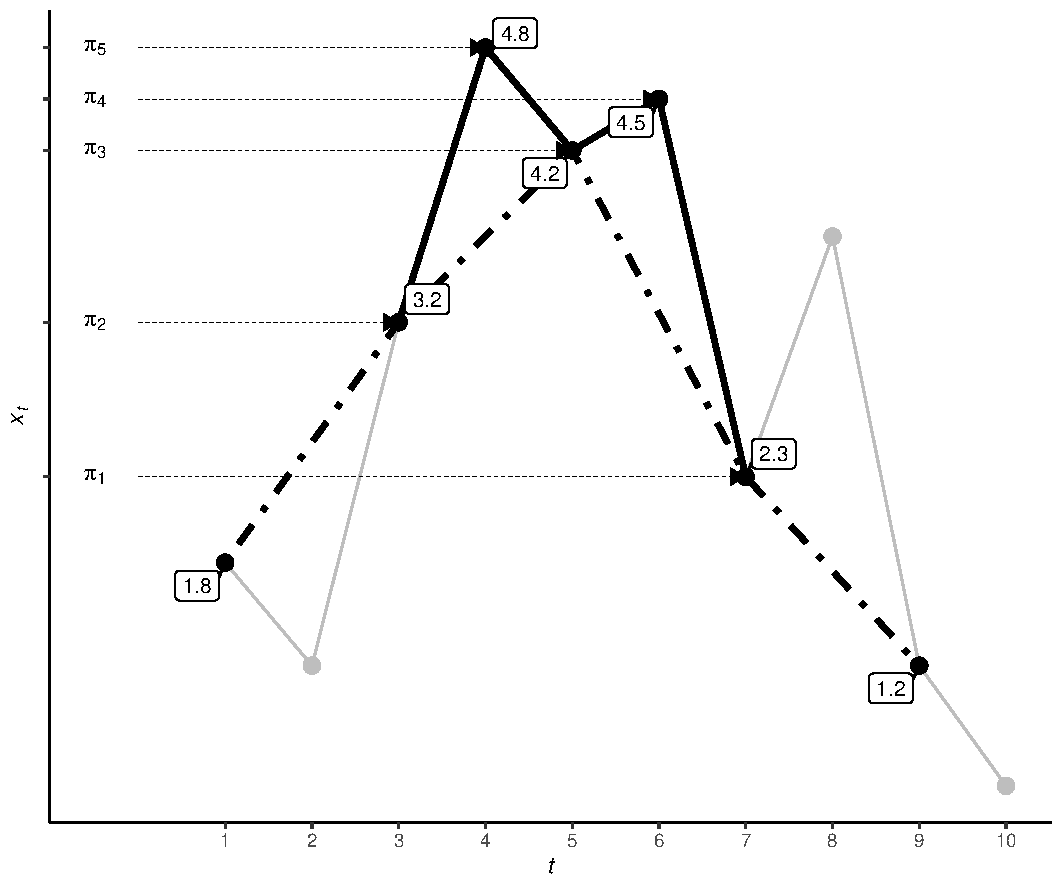
\includegraphics[width=.8\linewidth]{Figures/IntroBP}
	\caption{Illustration of the Bandt and Pompe coding\label{Fig:IntroBP}}
\end{figure}

The classical approach consists in analyzing the histogram of these patterns.
Denote $\Pi$ the sequence of symbols obtained by a given series $\mathbf{X}_t^{(D,\tau)}$.
The Bandt-Pompe probability distribution is the relative frequency of symbols in the series against $D!$ possible permutations of patterns $\{\widetilde\pi_t^D \}_{t = 1}^{D!}$:
\begin{equation}
p(\widetilde\pi_t^D) = \frac{\#\left \{t : t = 1, \dots, T-(D-1)\tau; \mathbf{X}_t^{(D,\tau)} \text{ is of type } \widetilde\pi_t^D\right \}}{T- (D-1)\tau},  
\end{equation}
that meets the conditions $p(\widetilde\pi_t^D) \ge 0$ and  $\sum_{i=1}^{D!} p(\widetilde\pi_t^D) = 1$.

Alternatively, one may form an oriented graph with the transitions from $\widetilde\pi_t^D$ to $\widetilde\pi_{t+1}^D$.
%%% ACF Aqui citar e comentar trabalhos que façam o grafo de transições

We modify this last approach by assigning weights to the edges related to the absolute difference of the observations.
This modification takes into account the scattering properties of the target, and leads to a good characterization of several types of textures.

The Ordinal Pattern Transition Graph ${G} = ({V}, {E})$ 
represents the transitions between two consecutive ordinal patterns over time $t$.
The vertices are the patterns, and the edges the transitions between them:
$V = \{v_{\widetilde\pi_t^D}\}$, and 
$E = \{(v_{\widetilde\pi_t^D}, v_{\widetilde\pi_{t+1}^D}): v_{\widetilde\pi_t^D}, v_{\widetilde\pi_{t+1}^D} \in V \}$~\cite{LearningandDistinguishingTimeSeriesDynamicsViaOrdinalPatternsTransitionGraphs2019}.

We find two main approaches in the literature in relation to the weight of edges.
Some authors employ unweighted edges~\cite{Kulp2016ordinal,McCullough2015lagged} representing only the existence of such transitions, while others apply the frequency of transitions~\cite{Sorrentino2015periodic,Zhang2017ConstructingOP}.
The weights $\mathbb{W} = \{w_{v_{\widetilde{\pi}^D_i}, v_{\widetilde\pi^D_j}}: v_{\widetilde\pi^D_i}, v_{\widetilde\pi^D_j} \in V \}$ assigned to each edge describe the chances of transition between two particular patterns $(v_{\widetilde\pi^D_i}, v_{\widetilde\pi^D_j})$ calculated by their respective relative frequencies, ie:
\begin{equation}
w_{v_{\widetilde\pi^D_i}, v_{\widetilde\pi^D_j}} = \frac{|\Pi_{\widetilde\pi^D_i,\widetilde\pi^D_j}|}{T-(D-1)\tau-1},
\end{equation}
where $|\Pi_{\widetilde\pi^D_i,\widetilde\pi^D_j}|$ is the number of transitions between patterns $\widetilde\pi^D_i$ and $\widetilde\pi^D_j$, $\sum_{v_{\widetilde\pi^D_i}, v_{\widetilde\pi^D_j}}w_{v_{\widetilde\pi^D_i}, v_{\widetilde\pi^D_j}} = 1$,
and the denominator is the number of transitions between sequential patterns in the series of motifs of length $T-(D-1)\tau$.

%%% "amplitude variances" está estranho. Quebre em duas sentenças.
Recent works propose a weighting in the calculation of relative frequencies for ordinal patterns with different amplitude variances, making them contribute differently to the final value of permutation entropy (PE) and thus incorporating amplitude change information within a set~\cite{Fadlallah2013Weightedpermutation}.
However, these methods do not consider the amplitude difference present in different time series, weighing them similarly when calculating the final value of their probabilities.
Therefore, data with different amplitudes but with similar variance dynamics are not discriminated, losing important information about the system dynamics.

To counterbalance these facts, we propose a modification of the current ordinal pattern transition graph by incorporating meaningful time series information.

Our proposal, henceforth referred to as Weighted Amplitude Transition Graph (WATG), incorporates the absolute difference between the observations that produced the patterns.

First, each $\mathcal{X}$ time series is scaled to $[0, 1]$, since we are interested in a metric able to compare data sets:
\begin{equation}
 \frac{x_i - x_{\min}}{x_{\max} - x_{\min}} \longmapsto x_i,
\end{equation}
where $x_{\min}$ and $x_{\max}$ are, respectively, the minimum and maximum values of the series.

Each $\mathbf{X}^{(D, \tau)}_t$ vector is associated with a weight $\beta_t$ that measures the largest difference between its elements:
\begin{equation}
\beta_t = \max\{x_i - x_j\},
\end{equation}
where $x_i, x_j \in \mathbf{X}^{(D, \tau)}_t$.

Traditionally, the transition graph assigns uniform weight to each transition between patterns and normalizes the result obtained by dividing by the total transitions.
In this modification, the $w_{v_{\widetilde\pi^D_i}, v_{\widetilde\pi^D_j}}$ weights assigned to each edge depict the amplitude difference observed in the transition.
So we have that:	
\begin{equation}
w_{v_{\widetilde \pi^D_i}, v_{\widetilde \pi^D_j}} =  \sum_{i : \{\mathbf{X}^{(D,\tau)}_t \mapsto \widetilde\pi^D_i\}} \sum_{j : \{\mathbf{X}^{(D,\tau)}_t \mapsto \widetilde\pi^D_j\}} |\beta_i - \beta_j| .
\end{equation}

Thus, the probability distribution taken from the weighted amplitude transition graph is given as follows:	
\begin{align}
&\left\{\begin{array}{l}
\lambda_{v_{\widetilde\pi^D_i}, v_{\widetilde\pi^D_j}} = 1, \text{ if } (v_{\widetilde\pi^D_i}, v_{\widetilde\pi^D_j}) \in {E} \\
\lambda_{v_{\widetilde\pi^D_i}, v_{\widetilde\pi^D_j}} = 0, \text{ otherwise}.
\end{array}\right. \\
%
&p(\widetilde\pi^D_i, \widetilde\pi^D_j) = \frac{\lambda_{v_{\widetilde\pi^D_i}, v_{\widetilde\pi^D_j}} \cdot w_{v_{\widetilde\pi^D_i}, v_{\widetilde\pi^D_j}}}{\sum_{v_{\widetilde\pi^D_a}, v_{\widetilde\pi^D_b}} w_{v_{\widetilde\pi^D_a}, v_{\widetilde\pi^D_b}}}.
\end{align}

Note that the conditions $p(\widetilde\pi^D_i, \widetilde\pi^D_j) \ge 0$ e $\sum_{\widetilde\pi^D_i, \widetilde\pi^D_j} p(\widetilde\pi^D_i, \widetilde\pi^D_j) = 1$ are satisfied.

Series with uniform amplitudes have edges with probability of occurrence well distributed along the graph, while those with large peaks have edges with probability of occurrence much higher than the others.

\begin{figure}[hbt]
	\centering
	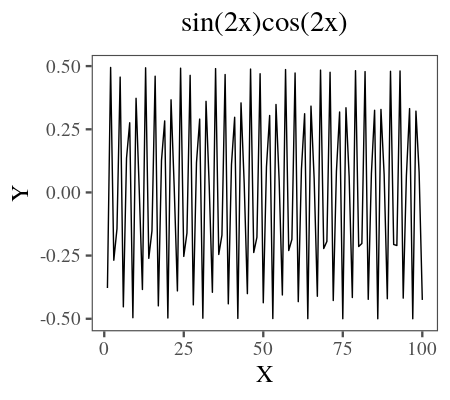
\includegraphics[width=.45\linewidth]{Figures/plotsincos.png}
	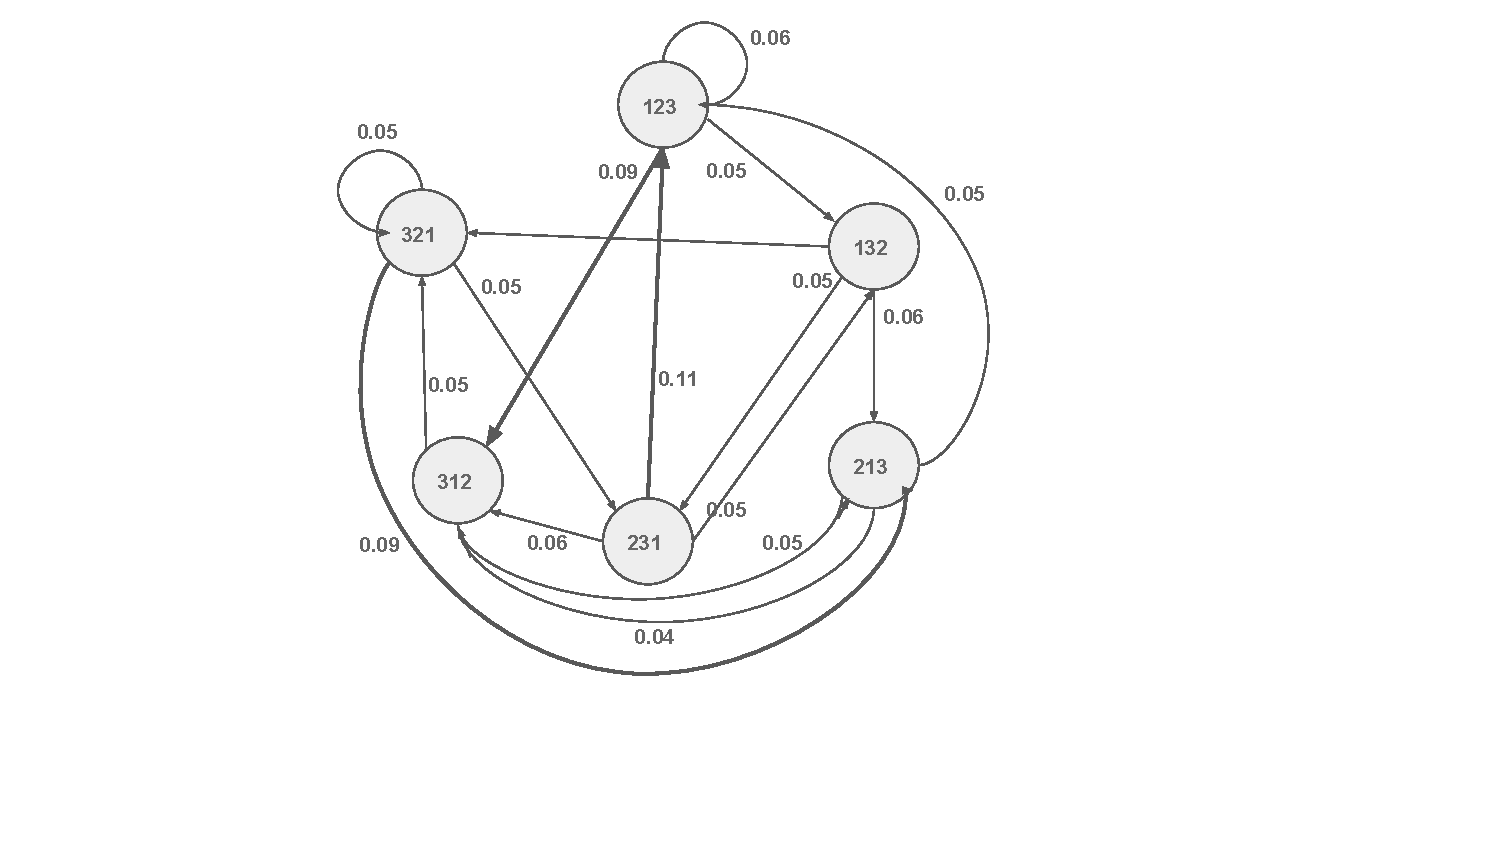
\includegraphics[width=.4\linewidth]{Figures/graph.pdf}
	\caption{Example of (a) the first 100 samples of the $\sin (2x)  \cos (2x)$ series and (b) the WATG for the series with $D = 3$ and $\tau = 1$}\label{fig:series}
\end{figure} 

\subsection{Information-Theoretic Descriptors}\label{HC}

Entropy measures the disorder or unpredictability of a system characterized by a probability measure $\mathbb{P}$.

Let $\mathbb{P} = \{p_{(\widetilde\pi^D_1, \widetilde\pi^D_1)}, p_{(\widetilde\pi^D_1, \widetilde\pi^D_2)}, \dots, p_{(\widetilde\pi^D_{D!}, \widetilde\pi^D_{D!})} \} = \{p_1,\dots,p_{D!^2}\}$ be the probability distribution taken from the time series weighted amplitude transition graph $\mathbb{X}$.
The normalized Shannon entropy is given by:	
\begin{equation}
H(\mathbb{P}) = -\frac1{2\log D!}\sum_{\ell=1}^{D!^2} p_{\ell} \log p_{\ell} .
\label{eq:Entropia}
\end{equation}

The ability of the entropy to capture system properties is limited, so it is necessary to use it in conjunction with other des\-criptors to perform a more complete analysis.
Other interesting measures are distances between the probability function $\mathbb{P}$ and a probability measure that describes a non-informative process, typically the uniform distribution.

The Jensen-Shannon distance to the uniform distribution $\mathbb{U} = (\frac{1}{D!^2}, \dots, \frac{1}{D!^2})$ is a measure of how similar the underlying dynamics are to a process without information; it is calculated as:
\begin{equation}
Q'(\mathbb{P}, \mathbb{U}) = \sum_{\ell=1}^{D!^2} \Big(p_\ell \log\frac{p_\ell}{u_\ell} +
u_\ell \log\frac{u_\ell}{p_\ell}
\Big).
\end{equation}
This quantity is also called ``disequilibrium.''
The normalized disequilibrium is $ Q=Q'/\max\{Q'\}$.

Conversely to entropy, statistical complexity seeks to find interaction and dependence structures among the elements of a given series, being an extremely important factor in the study of dynamic systems.

The Statistical Complexity is then defined as~\cite{Lamberti2004}:
\begin{equation}
C(\mathbb{P}, \mathbb{U}) = H(\mathbb{P}) Q(\mathbb{P}, \mathbb{U}).
\end{equation}

In our analysis, each time series can then be described by a point $(H(\mathbb{P}), C(\mathbb{P}, \mathbb{U}))$.
The set of all pairs $(H(\mathbb{P}), C(\mathbb{P}, \mathbb{U}))$ for any time series described by patterns of length $D$ lies in a compact subset of $\mathbbm R^2$: the Entropy-Complexity plane. 

Through such a tool it is possible to discover the nature of the series, determining if it corresponds to a chaotic (or other deterministic dynamics) or stochastic sequences.

\section{Textural classification of SAR regions}\label{SAR}

Widely used in recognizing geographical features and patterns, synthetic aperture radar (SAR) images are rich in texture information.
For this analysis, we will use the HH intensity band of three different region SAR images with uninhabited aerial vehicle (UAVSAR) SAR data, which provide fully polarimetric SAR observations:

\begin{itemize}
	\item Sierra del Lacandon National Park, Guatemala (acquired on April 10, 2015)\footnote{\protect{\url{https://uavsar.jpl.nasa.gov/cgi-bin/product.pl?jobName=Lacand_30202_15043_006_150410_L090_CX_01\#dados}}};
	\item Cape Canaveral Ocean Regions (acquired on September 22, 2016);
	\item Urban area of the city of Munich, Germany (acquired on June 5, 2015)\footnote{\protect{\url{https://uavsar.jpl.nasa.gov/cgi-bin/product.pl?jobName=munich_19417_15088_002_150605_L090_CX_01\#data}}}.
\end{itemize}
We will use in this work $160$ samples of size $128 \times 128$, with the following configuration:
$40$ samples from Guatemalan forest regions;
$80$ samples from the oceanic regions of Cape Canaveral, where they were divided into two types that have distinct contrast information; and
$40$ samples of urban regions of the city of Munich.
Figure ~\ref{fig:RegionsSAR} shows examples of each of them.

\begin{figure}[hbt]
	\centering
	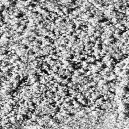
\includegraphics[width=.23\linewidth]{Figures/guatemalaflorest}
	
\includegraphics[width=.23\linewidth]{Figures/Cape1}
	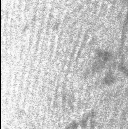
\includegraphics[width=.23\linewidth]{Figures/Cape2}
	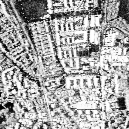
\includegraphics[width=.23\linewidth]{Figures/munichUrban}	
	\caption{Types of regions analyzed: Forest, Sea Type~1, Sea Type~2, and Urban.}\label{fig:RegionsSAR}
\end{figure} 

Since the symbolization process is invariant to monotonous transformations and resistant to contamination effects, contrast chan\-ges are not capable of causing changes in the final results obtained by the descriptors.
Thus, the different types of oceanic regions considered in this work were studied as a single more general class.

Figure~\ref{fig:AmplitudeSAR} shows examples of forest, sea and urban samples as time series, after the linearization process.

\begin{figure}[hbt]
	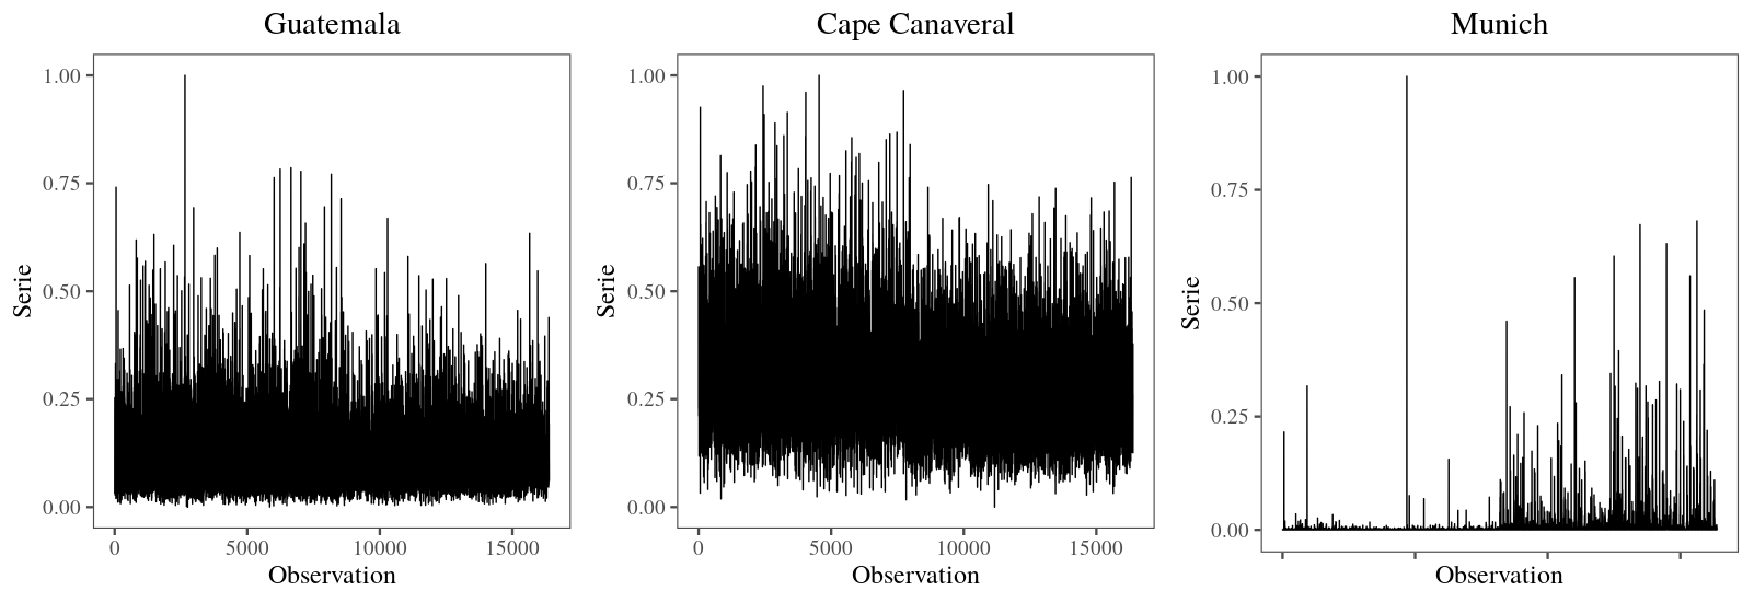
\includegraphics[width=\columnwidth]{Figures/SAR_signal.pdf}
	\caption{Analysis of the amplitude of the different types of regions: (a) Oceanic Region; (b) Forest Regions and (c) Urban Regions}
	\label{fig:AmplitudeSAR}
\end{figure} 

\section{Expected results}\label{sec:results}

The main contributions already achieved are:
(i)~a time series discrimination technique with different amplitude information, and
(ii)~a methodology for characterization of regions in SAR images, which proved to be adequate for the proposed data set.
In addition, we have preliminary results from quantitative analysis, indicating that such method has a good performance in SAR texture classification.

Following the evaluation of this new metric, two studies are planned: 
%%% A imputação não faz muito sentido, já que trabalhamos com imagens em formato float ou double. Ela faria sentido se mencionasse degradações da imagem que levem a dados faltantes.
the impact analysis of data imputation methods, and 
the prediction and simulation of events, both using transition graphs.

Exploratory work to study the power of reconstruction of time series data imputation techniques is now in its early stages.
We hope that with the use of transition graphs we will be able to contrast the impacts caused by the different approaches and be able to measure which one can most effectively describe the original series, for this we will use the Kullback-Leibler divergence.

Finally, we plan to conduct a study of ordinal patterns with transition graphs and Markov Chains.
The purpose is to combine the evidence of the time series, its ordinal patterns, and the transition graph to make simulations and predictions about the series.
One of the innovations of this work is to address one of the limitations of ordinal pattern-based time series analysis techniques that so far do not allow forecasting or simulations.


\section{Schedule and checkpoints}\label{sec:checkpoint}

This work is in its first year (second semester). 
As mentioned earlier, the initial research steps have already been taken.
The first submission to a conference in this context was made at the Latin American GRSS \& ISPRS Remote Sensing Conference, on the proposal for characterization of SAR images.

In the next steps, we plan:
(1)~conduct a literature review of current SAR image texture classification models;
(2)~study and propose an amplitude-based time series classification model;
(3)~investigate the characterization of transition graphs using the Kullback-Leibler divergence; 
(4)~study and design the transition graph prediction and event simulation algorithm; 
(5)~publish the scientific results obtained with this work (we aim at a publication in the IEEE Transactions on Geoscience and Remote Sensing); and
(6)~write and present this dissertation.

Table~\ref{Tab:Schedule} presents an estimated schedule for the aforementioned steps over a period of twelve months.

%%% ACF Faça um projeto no ProjectLibre, e transcreva as datas usando \usepackage{pgfgantt}
\begin{table}[hbt]
\caption{Monthly agenda for 2020}\label{Tab:Schedule}
\label{tab:agenda}
    \resizebox{\columnwidth}{!}{%
        \begin{tabular}{@{}lcccccccccccc@{}}
        \toprule
         & \textbf{Jan} & \textbf{Feb} & \textbf{Mar} & \textbf{Apr} & \textbf{May} & \multicolumn{1}{l}{\textbf{Jun}} & \multicolumn{1}{l}{\textbf{Jul}} & \multicolumn{1}{l}{\textbf{Aug}} & \multicolumn{1}{l}{\textbf{Sep}} & \multicolumn{1}{l}{\textbf{Oct}} & \multicolumn{1}{l}{\textbf{Nov}} & \multicolumn{1}{l}{\textbf{Dec}} \\ \midrule
        \multicolumn{1}{c}{\textbf{1}} & X & & & & & & & & & &  &  \\
        \multicolumn{1}{c}{\textbf{2}} & X & X &  &  &  &  &  &  &  &  &  &  \\
        \multicolumn{1}{c}{\textbf{3}} &  &  & X & X & X & & & & & &  &  \\
        \multicolumn{1}{c}{\textbf{4}} &  & & & & & X & X & X & & &  &  \\
        \multicolumn{1}{c}{\textbf{5}} &  &  &  & & & & & & X & X & X & X \\
        \multicolumn{1}{c}{\textbf{6}} &  &  &  & & & & & & X & X & X & X \\ \bottomrule
        \end{tabular}
    }
\end{table}

\section{Final remarks}\label{sec:final}

%\todo[inline]{Isso não é um paper}
%Done
This proposal presents the dissertation project entitled ``A study about ordinal patterns transition graphs.'' 
We argue that the information extracted from the ordinal transition graphs provides relevant details about the dynamics of the system that governs the time series, being an important characterization tool.

Therefore, the main expected contributions to this work are:
(i)~the proposal of a methodology of characterization of time series with different amplitudes,
(ii)~the evaluation of the method in relation to the others proposed in the literature, 
(iii)~the proposed algorithm for evaluating the imputation techniques given, 
(iv)~the proposal of a time series simulation and prediction methodology based on transition graphs and Markov chains.

%%% ACF Não entendi esta última frase
We present the key elements needed to achieve the above contributions.

% ======================================================================
	
\bibliographystyle{abbrv}
\bibliography{../../Common/references.bib}
	
\end{document}